\documentclass[1p]{elsarticle_modified}
%\bibliographystyle{elsarticle-num}

%\usepackage[colorlinks]{hyperref}
%\usepackage{abbrmath_seonhwa} %\Abb, \Ascr, \Acal ,\Abf, \Afrak
\usepackage{amsfonts}
\usepackage{amssymb}
\usepackage{amsmath}
\usepackage{amsthm}
\usepackage{scalefnt}
\usepackage{amsbsy}
\usepackage{kotex}
\usepackage{caption}
\usepackage{subfig}
\usepackage{color}
\usepackage{graphicx}
\usepackage{xcolor} %% white, black, red, green, blue, cyan, magenta, yellow
\usepackage{float}
\usepackage{setspace}
\usepackage{hyperref}

\usepackage{tikz}
\usetikzlibrary{arrows}

\usepackage{multirow}
\usepackage{array} % fixed length table
\usepackage{hhline}

%%%%%%%%%%%%%%%%%%%%%
\makeatletter
\renewcommand*\env@matrix[1][\arraystretch]{%
	\edef\arraystretch{#1}%
	\hskip -\arraycolsep
	\let\@ifnextchar\new@ifnextchar
	\array{*\c@MaxMatrixCols c}}
\makeatother %https://tex.stackexchange.com/questions/14071/how-can-i-increase-the-line-spacing-in-a-matrix
%%%%%%%%%%%%%%%

\usepackage[normalem]{ulem}

\newcommand{\msout}[1]{\ifmmode\text{\sout{\ensuremath{#1}}}\else\sout{#1}\fi}
%SOURCE: \msout is \stkout macro in https://tex.stackexchange.com/questions/20609/strikeout-in-math-mode

\newcommand{\cancel}[1]{
	\ifmmode
	{\color{red}\msout{#1}}
	\else
	{\color{red}\sout{#1}}
	\fi
}

\newcommand{\add}[1]{
	{\color{blue}\uwave{#1}}
}

\newcommand{\replace}[2]{
	\ifmmode
	{\color{red}\msout{#1}}{\color{blue}\uwave{#2}}
	\else
	{\color{red}\sout{#1}}{\color{blue}\uwave{#2}}
	\fi
}

\newcommand{\Sol}{\mathcal{S}} %segment
\newcommand{\D}{D} %diagram
\newcommand{\A}{\mathcal{A}} %arc


%%%%%%%%%%%%%%%%%%%%%%%%%%%%%5 test

\def\sl{\operatorname{\textup{SL}}(2,\Cbb)}
\def\psl{\operatorname{\textup{PSL}}(2,\Cbb)}
\def\quan{\mkern 1mu \triangleright \mkern 1mu}

\theoremstyle{definition}
\newtheorem{thm}{Theorem}[section]
\newtheorem{prop}[thm]{Proposition}
\newtheorem{lem}[thm]{Lemma}
\newtheorem{ques}[thm]{Question}
\newtheorem{cor}[thm]{Corollary}
\newtheorem{defn}[thm]{Definition}
\newtheorem{exam}[thm]{Example}
\newtheorem{rmk}[thm]{Remark}
\newtheorem{alg}[thm]{Algorithm}

\newcommand{\I}{\sqrt{-1}}
\begin{document}

%\begin{frontmatter}
%
%\title{Boundary parabolic representations of knots up to 8 crossings}
%
%%% Group authors per affiliation:
%\author{Yunhi Cho} 
%\address{Department of Mathematics, University of Seoul, Seoul, Korea}
%\ead{yhcho@uos.ac.kr}
%
%
%\author{Seonhwa Kim} %\fnref{s_kim}}
%\address{Center for Geometry and Physics, Institute for Basic Science, Pohang, 37673, Korea}
%\ead{ryeona17@ibs.re.kr}
%
%\author{Hyuk Kim}
%\address{Department of Mathematical Sciences, Seoul National University, Seoul 08826, Korea}
%\ead{hyukkim@snu.ac.kr}
%
%\author{Seokbeom Yoon}
%\address{Department of Mathematical Sciences, Seoul National University, Seoul, 08826,  Korea}
%\ead{sbyoon15@snu.ac.kr}
%
%\begin{abstract}
%We find all boundary parabolic representation of knots up to 8 crossings.
%
%\end{abstract}
%\begin{keyword}
%    \MSC[2010] 57M25 
%\end{keyword}
%
%\end{frontmatter}

%\linenumbers
%\tableofcontents
%
\newcommand\colored[1]{\textcolor{white}{\rule[-0.35ex]{0.8em}{1.4ex}}\kern-0.8em\color{red} #1}%
%\newcommand\colored[1]{\textcolor{white}{ #1}\kern-2.17ex	\textcolor{white}{ #1}\kern-1.81ex	\textcolor{white}{ #1}\kern-2.15ex\color{red}#1	}

{\Large $\underline{12a_{0292}~(K12a_{0292})}$}

\setlength{\tabcolsep}{10pt}
\renewcommand{\arraystretch}{1.6}
\vspace{1cm}\begin{tabular}{m{100pt}>{\centering\arraybackslash}m{274pt}}
\multirow{5}{120pt}{
	\centering
	\includegraphics[width=112pt]{../../../GIT/diagram.site/Diagrams/png/1093_12a_0292.png}\\
\ \ \ A knot diagram\footnotemark}&
\allowdisplaybreaks
\textbf{Linearized knot diagam} \\
\cline{2-2}
 &
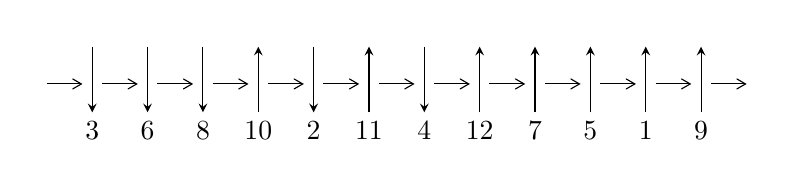
\begin{tikzpicture}[x=20pt, y=17pt]
	% nodes
	\node (C0) at (0, 0) {};
	\node (C1) at (1, 0) {};
	\node (C1U) at (1, +1) {};
	\node (C1D) at (1, -1) {3};

	\node (C2) at (2, 0) {};
	\node (C2U) at (2, +1) {};
	\node (C2D) at (2, -1) {6};

	\node (C3) at (3, 0) {};
	\node (C3U) at (3, +1) {};
	\node (C3D) at (3, -1) {8};

	\node (C4) at (4, 0) {};
	\node (C4U) at (4, +1) {};
	\node (C4D) at (4, -1) {10};

	\node (C5) at (5, 0) {};
	\node (C5U) at (5, +1) {};
	\node (C5D) at (5, -1) {2};

	\node (C6) at (6, 0) {};
	\node (C6U) at (6, +1) {};
	\node (C6D) at (6, -1) {11};

	\node (C7) at (7, 0) {};
	\node (C7U) at (7, +1) {};
	\node (C7D) at (7, -1) {4};

	\node (C8) at (8, 0) {};
	\node (C8U) at (8, +1) {};
	\node (C8D) at (8, -1) {12};

	\node (C9) at (9, 0) {};
	\node (C9U) at (9, +1) {};
	\node (C9D) at (9, -1) {7};

	\node (C10) at (10, 0) {};
	\node (C10U) at (10, +1) {};
	\node (C10D) at (10, -1) {5};

	\node (C11) at (11, 0) {};
	\node (C11U) at (11, +1) {};
	\node (C11D) at (11, -1) {1};

	\node (C12) at (12, 0) {};
	\node (C12U) at (12, +1) {};
	\node (C12D) at (12, -1) {9};
	\node (C13) at (13, 0) {};

	% arrows
	\draw[->,>={angle 60}]
	(C0) edge (C1) (C1) edge (C2) (C2) edge (C3) (C3) edge (C4) (C4) edge (C5) (C5) edge (C6) (C6) edge (C7) (C7) edge (C8) (C8) edge (C9) (C9) edge (C10) (C10) edge (C11) (C11) edge (C12) (C12) edge (C13) ;	\draw[->,>=stealth]
	(C1U) edge (C1D) (C2U) edge (C2D) (C3U) edge (C3D) (C4D) edge (C4U) (C5U) edge (C5D) (C6D) edge (C6U) (C7U) edge (C7D) (C8D) edge (C8U) (C9D) edge (C9U) (C10D) edge (C10U) (C11D) edge (C11U) (C12D) edge (C12U) ;
	\end{tikzpicture} \\
\hhline{~~} \\& 
\textbf{Solving Sequence} \\ \cline{2-2} 
 &
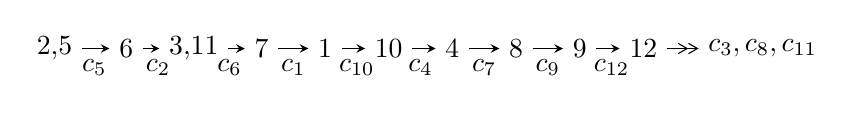
\begin{tikzpicture}[x=23pt, y=7pt]
	% node
	\node (A0) at (-1/8, 0) {2,5};
	\node (A1) at (1, 0) {6};
	\node (A2) at (33/16, 0) {3,11};
	\node (A3) at (25/8, 0) {7};
	\node (A4) at (33/8, 0) {1};
	\node (A5) at (41/8, 0) {10};
	\node (A6) at (49/8, 0) {4};
	\node (A7) at (57/8, 0) {8};
	\node (A8) at (65/8, 0) {9};
	\node (A9) at (73/8, 0) {12};
	\node (C1) at (1/2, -1) {$c_{5}$};
	\node (C2) at (3/2, -1) {$c_{2}$};
	\node (C3) at (21/8, -1) {$c_{6}$};
	\node (C4) at (29/8, -1) {$c_{1}$};
	\node (C5) at (37/8, -1) {$c_{10}$};
	\node (C6) at (45/8, -1) {$c_{4}$};
	\node (C7) at (53/8, -1) {$c_{7}$};
	\node (C8) at (61/8, -1) {$c_{9}$};
	\node (C9) at (69/8, -1) {$c_{12}$};
	\node (A10) at (11, 0) {$c_{3},c_{8},c_{11}$};

	% edge
	\draw[->,>=stealth]	
	(A0) edge (A1) (A1) edge (A2) (A2) edge (A3) (A3) edge (A4) (A4) edge (A5) (A5) edge (A6) (A6) edge (A7) (A7) edge (A8) (A8) edge (A9) ;
	\draw[->>,>={angle 60}]	
	(A9) edge (A10);
\end{tikzpicture} \\ 

\end{tabular} \\

\footnotetext{
The image of knot diagram is generated by the software ``\textbf{Draw programme}" developed by Andrew Bartholomew(\url{http://www.layer8.co.uk/maths/draw/index.htm\#Running-draw}), where we modified some parts for our purpose(\url{https://github.com/CATsTAILs/LinksPainter}).
}\phantom \\ \newline 
\centering \textbf{Ideals for irreducible components\footnotemark of $X_{\text{par}}$} 
 
\begin{align*}
I^u_{1}&=\langle 
8.95218\times10^{363} u^{136}+3.07057\times10^{364} u^{135}+\cdots+1.46551\times10^{364} b+1.37260\times10^{363},\\
\phantom{I^u_{1}}&\phantom{= \langle  }3.86404\times10^{367} u^{136}-1.31553\times10^{367} u^{135}+\cdots+1.06498\times10^{368} a-4.78268\times10^{370},\\
\phantom{I^u_{1}}&\phantom{= \langle  }u^{137}+3 u^{136}+\cdots+3010 u-169\rangle \\
I^u_{2}&=\langle 
-8 u^{28}+17 u^{27}+\cdots+b-27 u,\;-41 u^{28}+97 u^{27}+\cdots+a+59,\;u^{29}-3 u^{28}+\cdots-4 u+1\rangle \\
I^u_{3}&=\langle 
b-1,\;a-2,\;u+1\rangle \\
\\
\end{align*}
\raggedright * 3 irreducible components of $\dim_{\mathbb{C}}=0$, with total 167 representations.\\
\footnotetext{All coefficients of polynomials are rational numbers. But the coefficients are sometimes approximated in decimal forms when there is not enough margin.}
\newpage
\renewcommand{\arraystretch}{1}
\centering \section*{I. $I^u_{1}= \langle 8.95\times10^{363} u^{136}+3.07\times10^{364} u^{135}+\cdots+1.47\times10^{364} b+1.37\times10^{363},\;3.86\times10^{367} u^{136}-1.32\times10^{367} u^{135}+\cdots+1.06\times10^{368} a-4.78\times10^{370},\;u^{137}+3 u^{136}+\cdots+3010 u-169 \rangle$}
\flushleft \textbf{(i) Arc colorings}\\
\begin{tabular}{m{7pt} m{180pt} m{7pt} m{180pt} }
\flushright $a_{2}=$&$\begin{pmatrix}0\\u\end{pmatrix}$ \\
\flushright $a_{5}=$&$\begin{pmatrix}1\\0\end{pmatrix}$ \\
\flushright $a_{6}=$&$\begin{pmatrix}1\\u^2\end{pmatrix}$ \\
\flushright $a_{3}=$&$\begin{pmatrix}- u\\- u^3+u\end{pmatrix}$ \\
\flushright $a_{11}=$&$\begin{pmatrix}-0.362827 u^{136}+0.123526 u^{135}+\cdots-7278.77 u+449.086\\-0.610860 u^{136}-2.09523 u^{135}+\cdots-140.956 u-0.0936606\end{pmatrix}$ \\
\flushright $a_{7}=$&$\begin{pmatrix}8.71451 u^{136}+15.9346 u^{135}+\cdots+19901.9 u-1151.80\\-4.27979 u^{136}-6.45501 u^{135}+\cdots-1528.53 u+102.101\end{pmatrix}$ \\
\flushright $a_{1}=$&$\begin{pmatrix}u^3\\u^5- u^3+u\end{pmatrix}$ \\
\flushright $a_{10}=$&$\begin{pmatrix}0.248032 u^{136}+2.21876 u^{135}+\cdots-7137.82 u+449.179\\-0.610860 u^{136}-2.09523 u^{135}+\cdots-140.956 u-0.0936606\end{pmatrix}$ \\
\flushright $a_{4}=$&$\begin{pmatrix}3.38283 u^{136}+5.59457 u^{135}+\cdots+10568.1 u-625.048\\3.33673 u^{136}+9.05546 u^{135}+\cdots+19245.1 u-1033.06\end{pmatrix}$ \\
\flushright $a_{8}=$&$\begin{pmatrix}-12.0178 u^{136}-33.9406 u^{135}+\cdots-50266.6 u+2733.25\\13.2592 u^{136}+28.2260 u^{135}+\cdots+32710.1 u-1807.05\end{pmatrix}$ \\
\flushright $a_{9}=$&$\begin{pmatrix}6.13145 u^{136}+16.8119 u^{135}+\cdots+27710.4 u-1478.24\\-6.55283 u^{136}-15.1761 u^{135}+\cdots-17876.4 u+953.654\end{pmatrix}$ \\
\flushright $a_{12}=$&$\begin{pmatrix}-2.13161 u^{136}-3.37166 u^{135}+\cdots-11534.8 u+685.770\\0.694888 u^{136}+0.172607 u^{135}+\cdots+1710.79 u-115.185\end{pmatrix}$\\&\end{tabular}
\flushleft \textbf{(ii) Obstruction class $= -1$}\\~\\
\flushleft \textbf{(iii) Cusp Shapes $= 4.91390 u^{136}+17.0980 u^{135}+\cdots-4100.08 u+335.512$}\\~\\
\newpage\renewcommand{\arraystretch}{1}
\flushleft \textbf{(iv) u-Polynomials at the component}\newline \\
\begin{tabular}{m{50pt}|m{274pt}}
Crossings & \hspace{64pt}u-Polynomials at each crossing \\
\hline $$\begin{aligned}c_{1}\end{aligned}$$&$\begin{aligned}
&u^{137}+53 u^{136}+\cdots+3208982 u+28561
\end{aligned}$\\
\hline $$\begin{aligned}c_{2},c_{5}\end{aligned}$$&$\begin{aligned}
&u^{137}+3 u^{136}+\cdots+3010 u-169
\end{aligned}$\\
\hline $$\begin{aligned}c_{3},c_{7}\end{aligned}$$&$\begin{aligned}
&u^{137}+u^{136}+\cdots+481416 u-77291
\end{aligned}$\\
\hline $$\begin{aligned}c_{4},c_{10}\end{aligned}$$&$\begin{aligned}
&u^{137}+2 u^{136}+\cdots-8 u-1
\end{aligned}$\\
\hline $$\begin{aligned}c_{6}\end{aligned}$$&$\begin{aligned}
&u^{137}-3 u^{136}+\cdots+288732 u-248089
\end{aligned}$\\
\hline $$\begin{aligned}c_{8},c_{12}\end{aligned}$$&$\begin{aligned}
&u^{137}-9 u^{136}+\cdots+1468 u-271
\end{aligned}$\\
\hline $$\begin{aligned}c_{9}\end{aligned}$$&$\begin{aligned}
&u^{137}+11 u^{136}+\cdots-102807486 u-5507323
\end{aligned}$\\
\hline $$\begin{aligned}c_{11}\end{aligned}$$&$\begin{aligned}
&u^{137}-63 u^{136}+\cdots+597316 u-73441
\end{aligned}$\\
\hline
\end{tabular}\\~\\
\newpage\renewcommand{\arraystretch}{1}
\flushleft \textbf{(v) Riley Polynomials at the component}\newline \\
\begin{tabular}{m{50pt}|m{274pt}}
Crossings & \hspace{64pt}Riley Polynomials at each crossing \\
\hline $$\begin{aligned}c_{1}\end{aligned}$$&$\begin{aligned}
&y^{137}+75 y^{136}+\cdots+4313902139478 y-815730721
\end{aligned}$\\
\hline $$\begin{aligned}c_{2},c_{5}\end{aligned}$$&$\begin{aligned}
&y^{137}-53 y^{136}+\cdots+3208982 y-28561
\end{aligned}$\\
\hline $$\begin{aligned}c_{3},c_{7}\end{aligned}$$&$\begin{aligned}
&y^{137}+109 y^{136}+\cdots-59701913870 y-5973898681
\end{aligned}$\\
\hline $$\begin{aligned}c_{4},c_{10}\end{aligned}$$&$\begin{aligned}
&y^{137}-116 y^{136}+\cdots+78 y-1
\end{aligned}$\\
\hline $$\begin{aligned}c_{6}\end{aligned}$$&$\begin{aligned}
&y^{137}-35 y^{136}+\cdots-1429947953852 y-61548151921
\end{aligned}$\\
\hline $$\begin{aligned}c_{8},c_{12}\end{aligned}$$&$\begin{aligned}
&y^{137}-63 y^{136}+\cdots+597316 y-73441
\end{aligned}$\\
\hline $$\begin{aligned}c_{9}\end{aligned}$$&$\begin{aligned}
&y^{137}-43 y^{136}+\cdots+1343419781833972 y-30330606626329
\end{aligned}$\\
\hline $$\begin{aligned}c_{11}\end{aligned}$$&$\begin{aligned}
&y^{137}+37 y^{136}+\cdots+126623191148 y-5393580481
\end{aligned}$\\
\hline
\end{tabular}\\~\\
\newpage\flushleft \textbf{(vi) Complex Volumes and Cusp Shapes}
$$\begin{array}{c|c|c}  
\text{Solutions to }I^u_{1}& \I (\text{vol} + \sqrt{-1}CS) & \text{Cusp shape}\\
 \hline 
\begin{aligned}
u &= -0.805157 + 0.597246 I \\
a &= \phantom{-}0.94208 - 3.06119 I \\
b &= -1.200520 + 0.000228 I\end{aligned}
 & \phantom{-}7.32539 - 3.28612 I & \phantom{-0.000000 } 0 \\ \hline\begin{aligned}
u &= -0.805157 - 0.597246 I \\
a &= \phantom{-}0.94208 + 3.06119 I \\
b &= -1.200520 - 0.000228 I\end{aligned}
 & \phantom{-}7.32539 + 3.28612 I & \phantom{-0.000000 } 0 \\ \hline\begin{aligned}
u &= \phantom{-}0.582366 + 0.820362 I \\
a &= \phantom{-}0.513092 - 0.586948 I \\
b &= -1.259460 - 0.302714 I\end{aligned}
 & \phantom{-}3.86691 + 6.57125 I & \phantom{-0.000000 } 0 \\ \hline\begin{aligned}
u &= \phantom{-}0.582366 - 0.820362 I \\
a &= \phantom{-}0.513092 + 0.586948 I \\
b &= -1.259460 + 0.302714 I\end{aligned}
 & \phantom{-}3.86691 - 6.57125 I & \phantom{-0.000000 } 0 \\ \hline\begin{aligned}
u &= -0.420350 + 0.891795 I \\
a &= \phantom{-}0.470140 + 0.130367 I \\
b &= -1.280030 - 0.110876 I\end{aligned}
 & \phantom{-}6.43121 + 2.64534 I & \phantom{-0.000000 } 0 \\ \hline\begin{aligned}
u &= -0.420350 - 0.891795 I \\
a &= \phantom{-}0.470140 - 0.130367 I \\
b &= -1.280030 + 0.110876 I\end{aligned}
 & \phantom{-}6.43121 - 2.64534 I & \phantom{-0.000000 } 0 \\ \hline\begin{aligned}
u &= -0.795381 + 0.579290 I \\
a &= -0.049486 - 1.048380 I \\
b &= -1.81121 + 0.39041 I\end{aligned}
 & \phantom{-}3.92418 - 2.12374 I & \phantom{-0.000000 } 0 \\ \hline\begin{aligned}
u &= -0.795381 - 0.579290 I \\
a &= -0.049486 + 1.048380 I \\
b &= -1.81121 - 0.39041 I\end{aligned}
 & \phantom{-}3.92418 + 2.12374 I & \phantom{-0.000000 } 0 \\ \hline\begin{aligned}
u &= \phantom{-}0.729232 + 0.657074 I \\
a &= -0.115303 + 0.577631 I \\
b &= -1.362000 - 0.162869 I\end{aligned}
 & \phantom{-}3.43840 - 4.29669 I & \phantom{-0.000000 } 0 \\ \hline\begin{aligned}
u &= \phantom{-}0.729232 - 0.657074 I \\
a &= -0.115303 - 0.577631 I \\
b &= -1.362000 + 0.162869 I\end{aligned}
 & \phantom{-}3.43840 + 4.29669 I & \phantom{-0.000000 } 0\\
 \hline 
 \end{array}$$\newpage$$\begin{array}{c|c|c}  
\text{Solutions to }I^u_{1}& \I (\text{vol} + \sqrt{-1}CS) & \text{Cusp shape}\\
 \hline 
\begin{aligned}
u &= \phantom{-}0.995976 + 0.219993 I \\
a &= \phantom{-}0.48351 + 1.76669 I \\
b &= -0.382499 + 0.535032 I\end{aligned}
 & -5.05036 - 3.28202 I & \phantom{-0.000000 } 0 \\ \hline\begin{aligned}
u &= \phantom{-}0.995976 - 0.219993 I \\
a &= \phantom{-}0.48351 - 1.76669 I \\
b &= -0.382499 - 0.535032 I\end{aligned}
 & -5.05036 + 3.28202 I & \phantom{-0.000000 } 0 \\ \hline\begin{aligned}
u &= -0.768667 + 0.573669 I \\
a &= \phantom{-}1.350920 + 0.170266 I \\
b &= -1.321950 - 0.054992 I\end{aligned}
 & \phantom{-}5.55498 + 3.33530 I & \phantom{-0.000000 } 0 \\ \hline\begin{aligned}
u &= -0.768667 - 0.573669 I \\
a &= \phantom{-}1.350920 - 0.170266 I \\
b &= -1.321950 + 0.054992 I\end{aligned}
 & \phantom{-}5.55498 - 3.33530 I & \phantom{-0.000000 } 0 \\ \hline\begin{aligned}
u &= -0.762804 + 0.579753 I \\
a &= \phantom{-}0.82594 - 2.36747 I \\
b &= -1.50210 - 1.09316 I\end{aligned}
 & \phantom{-}6.00582 - 0.74830 I & \phantom{-0.000000 } 0 \\ \hline\begin{aligned}
u &= -0.762804 - 0.579753 I \\
a &= \phantom{-}0.82594 + 2.36747 I \\
b &= -1.50210 + 1.09316 I\end{aligned}
 & \phantom{-}6.00582 + 0.74830 I & \phantom{-0.000000 } 0 \\ \hline\begin{aligned}
u &= \phantom{-}0.937824 + 0.128756 I \\
a &= -0.55983 - 1.91038 I \\
b &= \phantom{-}0.328013 - 0.372403 I\end{aligned}
 & -4.63559 + 2.51248 I & \phantom{-0.000000 } 0 \\ \hline\begin{aligned}
u &= \phantom{-}0.937824 - 0.128756 I \\
a &= -0.55983 + 1.91038 I \\
b &= \phantom{-}0.328013 + 0.372403 I\end{aligned}
 & -4.63559 - 2.51248 I & \phantom{-0.000000 } 0 \\ \hline\begin{aligned}
u &= \phantom{-}0.460219 + 0.826570 I \\
a &= -0.535977 - 0.241258 I \\
b &= -0.292622 - 1.001390 I\end{aligned}
 & \phantom{-}3.86275 + 7.80029 I & \phantom{-0.000000 } 0 \\ \hline\begin{aligned}
u &= \phantom{-}0.460219 - 0.826570 I \\
a &= -0.535977 + 0.241258 I \\
b &= -0.292622 + 1.001390 I\end{aligned}
 & \phantom{-}3.86275 - 7.80029 I & \phantom{-0.000000 } 0\\
 \hline 
 \end{array}$$\newpage$$\begin{array}{c|c|c}  
\text{Solutions to }I^u_{1}& \I (\text{vol} + \sqrt{-1}CS) & \text{Cusp shape}\\
 \hline 
\begin{aligned}
u &= \phantom{-}0.835922 + 0.648923 I \\
a &= -1.33758 - 0.79335 I \\
b &= -0.20053 - 1.62112 I\end{aligned}
 & \phantom{-}6.59331 - 2.52785 I & \phantom{-0.000000 } 0 \\ \hline\begin{aligned}
u &= \phantom{-}0.835922 - 0.648923 I \\
a &= -1.33758 + 0.79335 I \\
b &= -0.20053 + 1.62112 I\end{aligned}
 & \phantom{-}6.59331 + 2.52785 I & \phantom{-0.000000 } 0 \\ \hline\begin{aligned}
u &= -0.536396 + 0.912755 I \\
a &= \phantom{-}0.442341 + 0.030875 I \\
b &= -1.45528 + 0.40733 I\end{aligned}
 & \phantom{-}6.77971 - 7.26834 I & \phantom{-0.000000 } 0 \\ \hline\begin{aligned}
u &= -0.536396 - 0.912755 I \\
a &= \phantom{-}0.442341 - 0.030875 I \\
b &= -1.45528 - 0.40733 I\end{aligned}
 & \phantom{-}6.77971 + 7.26834 I & \phantom{-0.000000 } 0 \\ \hline\begin{aligned}
u &= \phantom{-}0.756967 + 0.556841 I \\
a &= \phantom{-}0.179209 - 0.816030 I \\
b &= -1.323400 - 0.283899 I\end{aligned}
 & \phantom{-}5.45604 + 0.75830 I & \phantom{-0.000000 } 0 \\ \hline\begin{aligned}
u &= \phantom{-}0.756967 - 0.556841 I \\
a &= \phantom{-}0.179209 + 0.816030 I \\
b &= -1.323400 + 0.283899 I\end{aligned}
 & \phantom{-}5.45604 - 0.75830 I & \phantom{-0.000000 } 0 \\ \hline\begin{aligned}
u &= -0.613712 + 0.691576 I \\
a &= \phantom{-}0.152562 - 0.705237 I \\
b &= \phantom{-}0.043581 - 0.708646 I\end{aligned}
 & -0.12937 - 2.89825 I & \phantom{-0.000000 } 0 \\ \hline\begin{aligned}
u &= -0.613712 - 0.691576 I \\
a &= \phantom{-}0.152562 + 0.705237 I \\
b &= \phantom{-}0.043581 + 0.708646 I\end{aligned}
 & -0.12937 + 2.89825 I & \phantom{-0.000000 } 0 \\ \hline\begin{aligned}
u &= -0.885459 + 0.249630 I \\
a &= -0.638486 + 0.656935 I \\
b &= -0.446036 + 0.542795 I\end{aligned}
 & -1.49558 + 0.52853 I & \phantom{-0.000000 } 0 \\ \hline\begin{aligned}
u &= -0.885459 - 0.249630 I \\
a &= -0.638486 - 0.656935 I \\
b &= -0.446036 - 0.542795 I\end{aligned}
 & -1.49558 - 0.52853 I & \phantom{-0.000000 } 0\\
 \hline 
 \end{array}$$\newpage$$\begin{array}{c|c|c}  
\text{Solutions to }I^u_{1}& \I (\text{vol} + \sqrt{-1}CS) & \text{Cusp shape}\\
 \hline 
\begin{aligned}
u &= -0.903559 + 0.594068 I \\
a &= -1.56952 + 0.00075 I \\
b &= \phantom{-}1.321480 + 0.032747 I\end{aligned}
 & \phantom{-}7.00750 + 7.99825 I & \phantom{-0.000000 } 0 \\ \hline\begin{aligned}
u &= -0.903559 - 0.594068 I \\
a &= -1.56952 - 0.00075 I \\
b &= \phantom{-}1.321480 - 0.032747 I\end{aligned}
 & \phantom{-}7.00750 - 7.99825 I & \phantom{-0.000000 } 0 \\ \hline\begin{aligned}
u &= -0.906445 + 0.590629 I \\
a &= -0.30300 + 2.22630 I \\
b &= \phantom{-}1.76820 + 0.60307 I\end{aligned}
 & \phantom{-}3.56012 + 6.77597 I & \phantom{-0.000000 } 0 \\ \hline\begin{aligned}
u &= -0.906445 - 0.590629 I \\
a &= -0.30300 - 2.22630 I \\
b &= \phantom{-}1.76820 - 0.60307 I\end{aligned}
 & \phantom{-}3.56012 - 6.77597 I & \phantom{-0.000000 } 0 \\ \hline\begin{aligned}
u &= \phantom{-}0.858844 + 0.313988 I \\
a &= -0.088619 + 1.069430 I \\
b &= \phantom{-}1.361350 + 0.283896 I\end{aligned}
 & \phantom{-}5.33482 + 3.74361 I & \phantom{-0.000000 } 0 \\ \hline\begin{aligned}
u &= \phantom{-}0.858844 - 0.313988 I \\
a &= -0.088619 - 1.069430 I \\
b &= \phantom{-}1.361350 - 0.283896 I\end{aligned}
 & \phantom{-}5.33482 - 3.74361 I & \phantom{-0.000000 } 0 \\ \hline\begin{aligned}
u &= \phantom{-}0.493761 + 0.768951 I \\
a &= -0.550981 + 0.376015 I \\
b &= \phantom{-}1.232270 + 0.274925 I\end{aligned}
 & \phantom{-}2.23426 + 1.95781 I & \phantom{-0.000000 } 0 \\ \hline\begin{aligned}
u &= \phantom{-}0.493761 - 0.768951 I \\
a &= -0.550981 - 0.376015 I \\
b &= \phantom{-}1.232270 - 0.274925 I\end{aligned}
 & \phantom{-}2.23426 - 1.95781 I & \phantom{-0.000000 } 0 \\ \hline\begin{aligned}
u &= \phantom{-}0.363183 + 0.833917 I \\
a &= \phantom{-}0.0355355 + 0.0902461 I \\
b &= -1.273840 - 0.188516 I\end{aligned}
 & \phantom{-}6.39976 + 1.56844 I & \phantom{-0.000000 } 0 \\ \hline\begin{aligned}
u &= \phantom{-}0.363183 - 0.833917 I \\
a &= \phantom{-}0.0355355 - 0.0902461 I \\
b &= -1.273840 + 0.188516 I\end{aligned}
 & \phantom{-}6.39976 - 1.56844 I & \phantom{-0.000000 } 0\\
 \hline 
 \end{array}$$\newpage$$\begin{array}{c|c|c}  
\text{Solutions to }I^u_{1}& \I (\text{vol} + \sqrt{-1}CS) & \text{Cusp shape}\\
 \hline 
\begin{aligned}
u &= -0.926008 + 0.591810 I \\
a &= \phantom{-}0.876925 + 0.471655 I \\
b &= \phantom{-}1.74886 - 0.87662 I\end{aligned}
 & \phantom{-}5.48126 + 5.41757 I & \phantom{-0.000000 } 0 \\ \hline\begin{aligned}
u &= -0.926008 - 0.591810 I \\
a &= \phantom{-}0.876925 - 0.471655 I \\
b &= \phantom{-}1.74886 + 0.87662 I\end{aligned}
 & \phantom{-}5.48126 - 5.41757 I & \phantom{-0.000000 } 0 \\ \hline\begin{aligned}
u &= -0.925435 + 0.610641 I \\
a &= -0.35428 + 2.26738 I \\
b &= \phantom{-}1.207250 + 0.018699 I\end{aligned}
 & \phantom{-}5.02673 + 1.38814 I & \phantom{-0.000000 } 0 \\ \hline\begin{aligned}
u &= -0.925435 - 0.610641 I \\
a &= -0.35428 - 2.26738 I \\
b &= \phantom{-}1.207250 - 0.018699 I\end{aligned}
 & \phantom{-}5.02673 - 1.38814 I & \phantom{-0.000000 } 0 \\ \hline\begin{aligned}
u &= -0.734042 + 0.502418 I \\
a &= \phantom{-}0.94683 - 1.32163 I \\
b &= \phantom{-}0.200494 - 0.739966 I\end{aligned}
 & \phantom{-}1.65290 + 1.27822 I & \phantom{-0.000000 } 0 \\ \hline\begin{aligned}
u &= -0.734042 - 0.502418 I \\
a &= \phantom{-}0.94683 + 1.32163 I \\
b &= \phantom{-}0.200494 + 0.739966 I\end{aligned}
 & \phantom{-}1.65290 - 1.27822 I & \phantom{-0.000000 } 0 \\ \hline\begin{aligned}
u &= \phantom{-}0.885695 + 0.672060 I \\
a &= -0.322862 - 1.340580 I \\
b &= \phantom{-}1.123070 - 0.407962 I\end{aligned}
 & \phantom{-}2.99396 - 0.90542 I & \phantom{-0.000000 } 0 \\ \hline\begin{aligned}
u &= \phantom{-}0.885695 - 0.672060 I \\
a &= -0.322862 + 1.340580 I \\
b &= \phantom{-}1.123070 + 0.407962 I\end{aligned}
 & \phantom{-}2.99396 + 0.90542 I & \phantom{-0.000000 } 0 \\ \hline\begin{aligned}
u &= -0.979547 + 0.531619 I \\
a &= \phantom{-}0.129656 - 0.966748 I \\
b &= \phantom{-}0.154616 - 0.769501 I\end{aligned}
 & \phantom{-}0.82013 + 2.94411 I & \phantom{-0.000000 } 0 \\ \hline\begin{aligned}
u &= -0.979547 - 0.531619 I \\
a &= \phantom{-}0.129656 + 0.966748 I \\
b &= \phantom{-}0.154616 + 0.769501 I\end{aligned}
 & \phantom{-}0.82013 - 2.94411 I & \phantom{-0.000000 } 0\\
 \hline 
 \end{array}$$\newpage$$\begin{array}{c|c|c}  
\text{Solutions to }I^u_{1}& \I (\text{vol} + \sqrt{-1}CS) & \text{Cusp shape}\\
 \hline 
\begin{aligned}
u &= -0.714460 + 0.857758 I \\
a &= -0.197795 + 0.124690 I \\
b &= \phantom{-}1.50337 - 0.46402 I\end{aligned}
 & \phantom{-}12.58990 - 3.92968 I & \phantom{-0.000000 } 0 \\ \hline\begin{aligned}
u &= -0.714460 - 0.857758 I \\
a &= -0.197795 - 0.124690 I \\
b &= \phantom{-}1.50337 + 0.46402 I\end{aligned}
 & \phantom{-}12.58990 + 3.92968 I & \phantom{-0.000000 } 0 \\ \hline\begin{aligned}
u &= \phantom{-}0.947528 + 0.599587 I \\
a &= \phantom{-}0.25581 - 2.36909 I \\
b &= \phantom{-}1.207140 - 0.361511 I\end{aligned}
 & \phantom{-}4.80636 - 5.39144 I & \phantom{-0.000000 } 0 \\ \hline\begin{aligned}
u &= \phantom{-}0.947528 - 0.599587 I \\
a &= \phantom{-}0.25581 + 2.36909 I \\
b &= \phantom{-}1.207140 + 0.361511 I\end{aligned}
 & \phantom{-}4.80636 + 5.39144 I & \phantom{-0.000000 } 0 \\ \hline\begin{aligned}
u &= -1.110130 + 0.161489 I \\
a &= -0.47189 + 1.38956 I \\
b &= \phantom{-}0.136424 + 0.945028 I\end{aligned}
 & -3.43698 - 0.34927 I & \phantom{-0.000000 } 0 \\ \hline\begin{aligned}
u &= -1.110130 - 0.161489 I \\
a &= -0.47189 - 1.38956 I \\
b &= \phantom{-}0.136424 - 0.945028 I\end{aligned}
 & -3.43698 + 0.34927 I & \phantom{-0.000000 } 0 \\ \hline\begin{aligned}
u &= \phantom{-}0.718727 + 0.865772 I \\
a &= -0.519296 - 0.193775 I \\
b &= -0.024883 + 0.171220 I\end{aligned}
 & \phantom{-}5.24176 - 4.17178 I & \phantom{-0.000000 } 0 \\ \hline\begin{aligned}
u &= \phantom{-}0.718727 - 0.865772 I \\
a &= -0.519296 + 0.193775 I \\
b &= -0.024883 - 0.171220 I\end{aligned}
 & \phantom{-}5.24176 + 4.17178 I & \phantom{-0.000000 } 0 \\ \hline\begin{aligned}
u &= \phantom{-}0.845642 + 0.209874 I \\
a &= -0.00020 - 1.47019 I \\
b &= \phantom{-}1.48944 - 0.27192 I\end{aligned}
 & \phantom{-}3.35618 + 0.92289 I & \phantom{-0.000000 } 0 \\ \hline\begin{aligned}
u &= \phantom{-}0.845642 - 0.209874 I \\
a &= -0.00020 + 1.47019 I \\
b &= \phantom{-}1.48944 + 0.27192 I\end{aligned}
 & \phantom{-}3.35618 - 0.92289 I & \phantom{-0.000000 } 0\\
 \hline 
 \end{array}$$\newpage$$\begin{array}{c|c|c}  
\text{Solutions to }I^u_{1}& \I (\text{vol} + \sqrt{-1}CS) & \text{Cusp shape}\\
 \hline 
\begin{aligned}
u &= -1.011870 + 0.529443 I \\
a &= -0.777769 + 1.148430 I \\
b &= -0.080843 + 0.852716 I\end{aligned}
 & -3.12449 + 2.84870 I & \phantom{-0.000000 } 0 \\ \hline\begin{aligned}
u &= -1.011870 - 0.529443 I \\
a &= -0.777769 - 1.148430 I \\
b &= -0.080843 - 0.852716 I\end{aligned}
 & -3.12449 - 2.84870 I & \phantom{-0.000000 } 0 \\ \hline\begin{aligned}
u &= -1.140060 + 0.067440 I \\
a &= -1.083730 + 0.788776 I \\
b &= -0.986959 + 0.326375 I\end{aligned}
 & -3.15353 - 0.17714 I & \phantom{-0.000000 } 0 \\ \hline\begin{aligned}
u &= -1.140060 - 0.067440 I \\
a &= -1.083730 - 0.788776 I \\
b &= -0.986959 - 0.326375 I\end{aligned}
 & -3.15353 + 0.17714 I & \phantom{-0.000000 } 0 \\ \hline\begin{aligned}
u &= -0.549630 + 1.013530 I \\
a &= -0.369820 - 0.135073 I \\
b &= \phantom{-}1.43098 - 0.42597 I\end{aligned}
 & \phantom{-}9.2405 - 12.8750 I & \phantom{-0.000000 } 0 \\ \hline\begin{aligned}
u &= -0.549630 - 1.013530 I \\
a &= -0.369820 + 0.135073 I \\
b &= \phantom{-}1.43098 + 0.42597 I\end{aligned}
 & \phantom{-}9.2405 + 12.8750 I & \phantom{-0.000000 } 0 \\ \hline\begin{aligned}
u &= \phantom{-}1.014690 + 0.547849 I \\
a &= -0.390138 + 0.507725 I \\
b &= \phantom{-}0.163450 + 0.015988 I\end{aligned}
 & \phantom{-}0.84620 - 2.97680 I & \phantom{-0.000000 } 0 \\ \hline\begin{aligned}
u &= \phantom{-}1.014690 - 0.547849 I \\
a &= -0.390138 - 0.507725 I \\
b &= \phantom{-}0.163450 - 0.015988 I\end{aligned}
 & \phantom{-}0.84620 + 2.97680 I & \phantom{-0.000000 } 0 \\ \hline\begin{aligned}
u &= \phantom{-}0.641887 + 0.551583 I \\
a &= \phantom{-}0.388466 + 0.873075 I \\
b &= \phantom{-}0.182082 - 0.132393 I\end{aligned}
 & \phantom{-}1.99070 - 1.46530 I & \phantom{-0.000000 } 0 \\ \hline\begin{aligned}
u &= \phantom{-}0.641887 - 0.551583 I \\
a &= \phantom{-}0.388466 - 0.873075 I \\
b &= \phantom{-}0.182082 + 0.132393 I\end{aligned}
 & \phantom{-}1.99070 + 1.46530 I & \phantom{-0.000000 } 0\\
 \hline 
 \end{array}$$\newpage$$\begin{array}{c|c|c}  
\text{Solutions to }I^u_{1}& \I (\text{vol} + \sqrt{-1}CS) & \text{Cusp shape}\\
 \hline 
\begin{aligned}
u &= -0.867742 + 0.770476 I \\
a &= \phantom{-}1.39238 - 1.47624 I \\
b &= -1.240520 - 0.006387 I\end{aligned}
 & \phantom{-}8.87079 + 3.84557 I & \phantom{-0.000000 } 0 \\ \hline\begin{aligned}
u &= -0.867742 - 0.770476 I \\
a &= \phantom{-}1.39238 + 1.47624 I \\
b &= -1.240520 + 0.006387 I\end{aligned}
 & \phantom{-}8.87079 - 3.84557 I & \phantom{-0.000000 } 0 \\ \hline\begin{aligned}
u &= -1.160450 + 0.022793 I \\
a &= \phantom{-}1.22869 + 1.01050 I \\
b &= \phantom{-}1.076690 + 0.258704 I\end{aligned}
 & -2.25383 + 5.25220 I & \phantom{-0.000000 } 0 \\ \hline\begin{aligned}
u &= -1.160450 - 0.022793 I \\
a &= \phantom{-}1.22869 - 1.01050 I \\
b &= \phantom{-}1.076690 - 0.258704 I\end{aligned}
 & -2.25383 - 5.25220 I & \phantom{-0.000000 } 0 \\ \hline\begin{aligned}
u &= -1.116600 + 0.322148 I \\
a &= -0.005519 + 1.177000 I \\
b &= -0.179972 + 0.823837 I\end{aligned}
 & \phantom{-}0.361235 + 0.123400 I & \phantom{-0.000000 } 0 \\ \hline\begin{aligned}
u &= -1.116600 - 0.322148 I \\
a &= -0.005519 - 1.177000 I \\
b &= -0.179972 - 0.823837 I\end{aligned}
 & \phantom{-}0.361235 - 0.123400 I & \phantom{-0.000000 } 0 \\ \hline\begin{aligned}
u &= \phantom{-}1.031800 + 0.572120 I \\
a &= \phantom{-}0.15905 + 1.64340 I \\
b &= -1.216460 + 0.463784 I\end{aligned}
 & \phantom{-}0.71536 - 5.23431 I & \phantom{-0.000000 } 0 \\ \hline\begin{aligned}
u &= \phantom{-}1.031800 - 0.572120 I \\
a &= \phantom{-}0.15905 - 1.64340 I \\
b &= -1.216460 - 0.463784 I\end{aligned}
 & \phantom{-}0.71536 + 5.23431 I & \phantom{-0.000000 } 0 \\ \hline\begin{aligned}
u &= -0.895469 + 0.768409 I \\
a &= -1.47837 + 0.48380 I \\
b &= \phantom{-}1.285770 + 0.021386 I\end{aligned}
 & \phantom{-}8.78653 + 1.96366 I & \phantom{-0.000000 } 0 \\ \hline\begin{aligned}
u &= -0.895469 - 0.768409 I \\
a &= -1.47837 - 0.48380 I \\
b &= \phantom{-}1.285770 - 0.021386 I\end{aligned}
 & \phantom{-}8.78653 - 1.96366 I & \phantom{-0.000000 } 0\\
 \hline 
 \end{array}$$\newpage$$\begin{array}{c|c|c}  
\text{Solutions to }I^u_{1}& \I (\text{vol} + \sqrt{-1}CS) & \text{Cusp shape}\\
 \hline 
\begin{aligned}
u &= \phantom{-}0.485530 + 0.651974 I \\
a &= -0.603509 - 0.363535 I \\
b &= \phantom{-}1.186540 + 0.144046 I\end{aligned}
 & \phantom{-}2.28053 + 0.47722 I & \phantom{-0.000000 } 0 \\ \hline\begin{aligned}
u &= \phantom{-}0.485530 - 0.651974 I \\
a &= -0.603509 + 0.363535 I \\
b &= \phantom{-}1.186540 - 0.144046 I\end{aligned}
 & \phantom{-}2.28053 - 0.47722 I & \phantom{-0.000000 } 0 \\ \hline\begin{aligned}
u &= -1.005540 + 0.634699 I \\
a &= \phantom{-}0.799485 - 1.090420 I \\
b &= \phantom{-}0.064117 - 0.798768 I\end{aligned}
 & -1.28991 + 8.03213 I & \phantom{-0.000000 } 0 \\ \hline\begin{aligned}
u &= -1.005540 - 0.634699 I \\
a &= \phantom{-}0.799485 + 1.090420 I \\
b &= \phantom{-}0.064117 + 0.798768 I\end{aligned}
 & -1.28991 - 8.03213 I & \phantom{-0.000000 } 0 \\ \hline\begin{aligned}
u &= \phantom{-}0.790095 + 0.169162 I \\
a &= \phantom{-}1.85284 - 0.18452 I \\
b &= \phantom{-}1.119750 + 0.581126 I\end{aligned}
 & \phantom{-}1.46263 + 2.58621 I & \phantom{-0.000000 } 0 \\ \hline\begin{aligned}
u &= \phantom{-}0.790095 - 0.169162 I \\
a &= \phantom{-}1.85284 + 0.18452 I \\
b &= \phantom{-}1.119750 - 0.581126 I\end{aligned}
 & \phantom{-}1.46263 - 2.58621 I & \phantom{-0.000000 } 0 \\ \hline\begin{aligned}
u &= \phantom{-}1.041870 + 0.583418 I \\
a &= \phantom{-}0.78559 + 1.40487 I \\
b &= -0.397212 + 1.265350 I\end{aligned}
 & -0.75701 - 7.14868 I & \phantom{-0.000000 } 0 \\ \hline\begin{aligned}
u &= \phantom{-}1.041870 - 0.583418 I \\
a &= \phantom{-}0.78559 - 1.40487 I \\
b &= -0.397212 - 1.265350 I\end{aligned}
 & -0.75701 + 7.14868 I & \phantom{-0.000000 } 0 \\ \hline\begin{aligned}
u &= \phantom{-}0.371154 + 0.691685 I \\
a &= -1.114760 - 0.578166 I \\
b &= -0.165702 + 0.273462 I\end{aligned}
 & \phantom{-}4.41381 + 2.76426 I & \phantom{-0.000000 } 0 \\ \hline\begin{aligned}
u &= \phantom{-}0.371154 - 0.691685 I \\
a &= -1.114760 + 0.578166 I \\
b &= -0.165702 - 0.273462 I\end{aligned}
 & \phantom{-}4.41381 - 2.76426 I & \phantom{-0.000000 } 0\\
 \hline 
 \end{array}$$\newpage$$\begin{array}{c|c|c}  
\text{Solutions to }I^u_{1}& \I (\text{vol} + \sqrt{-1}CS) & \text{Cusp shape}\\
 \hline 
\begin{aligned}
u &= -1.229050 + 0.049572 I \\
a &= \phantom{-}0.341295 - 1.278050 I \\
b &= -0.145670 - 0.890855 I\end{aligned}
 & -1.99459 - 5.49143 I & \phantom{-0.000000 } 0 \\ \hline\begin{aligned}
u &= -1.229050 - 0.049572 I \\
a &= \phantom{-}0.341295 + 1.278050 I \\
b &= -0.145670 + 0.890855 I\end{aligned}
 & -1.99459 + 5.49143 I & \phantom{-0.000000 } 0 \\ \hline\begin{aligned}
u &= \phantom{-}1.069700 + 0.633929 I \\
a &= \phantom{-}0.16348 + 2.01580 I \\
b &= -1.251860 + 0.382869 I\end{aligned}
 & \phantom{-}0.53910 - 7.26662 I & \phantom{-0.000000 } 0 \\ \hline\begin{aligned}
u &= \phantom{-}1.069700 - 0.633929 I \\
a &= \phantom{-}0.16348 - 2.01580 I \\
b &= -1.251860 - 0.382869 I\end{aligned}
 & \phantom{-}0.53910 + 7.26662 I & \phantom{-0.000000 } 0 \\ \hline\begin{aligned}
u &= -1.001310 + 0.737994 I \\
a &= \phantom{-}0.34453 - 1.90902 I \\
b &= -1.50917 - 0.56211 I\end{aligned}
 & \phantom{-}11.6929 + 9.8554 I & \phantom{-0.000000 } 0 \\ \hline\begin{aligned}
u &= -1.001310 - 0.737994 I \\
a &= \phantom{-}0.34453 + 1.90902 I \\
b &= -1.50917 + 0.56211 I\end{aligned}
 & \phantom{-}11.6929 - 9.8554 I & \phantom{-0.000000 } 0 \\ \hline\begin{aligned}
u &= \phantom{-}0.960728 + 0.809195 I \\
a &= \phantom{-}0.343260 - 0.121407 I \\
b &= -0.0794187 - 0.0837330 I\end{aligned}
 & \phantom{-}4.55247 - 1.99359 I & \phantom{-0.000000 } 0 \\ \hline\begin{aligned}
u &= \phantom{-}0.960728 - 0.809195 I \\
a &= \phantom{-}0.343260 + 0.121407 I \\
b &= -0.0794187 + 0.0837330 I\end{aligned}
 & \phantom{-}4.55247 + 1.99359 I & \phantom{-0.000000 } 0 \\ \hline\begin{aligned}
u &= \phantom{-}0.709570 + 0.222459 I \\
a &= -2.90146 + 1.84149 I \\
b &= -1.090360 + 0.387055 I\end{aligned}
 & \phantom{-}5.72206 - 6.07019 I & \phantom{-0.000000 } 0 \\ \hline\begin{aligned}
u &= \phantom{-}0.709570 - 0.222459 I \\
a &= -2.90146 - 1.84149 I \\
b &= -1.090360 - 0.387055 I\end{aligned}
 & \phantom{-}5.72206 + 6.07019 I & \phantom{-0.000000 } 0\\
 \hline 
 \end{array}$$\newpage$$\begin{array}{c|c|c}  
\text{Solutions to }I^u_{1}& \I (\text{vol} + \sqrt{-1}CS) & \text{Cusp shape}\\
 \hline 
\begin{aligned}
u &= \phantom{-}1.062540 + 0.686303 I \\
a &= -0.26131 - 2.14684 I \\
b &= \phantom{-}1.255050 - 0.362414 I\end{aligned}
 & \phantom{-}2.42242 - 12.22940 I & \phantom{-0.000000 } 0 \\ \hline\begin{aligned}
u &= \phantom{-}1.062540 - 0.686303 I \\
a &= -0.26131 + 2.14684 I \\
b &= \phantom{-}1.255050 + 0.362414 I\end{aligned}
 & \phantom{-}2.42242 + 12.22940 I & \phantom{-0.000000 } 0 \\ \hline\begin{aligned}
u &= \phantom{-}0.409639 + 0.609308 I \\
a &= \phantom{-}0.540581 - 0.186551 I \\
b &= \phantom{-}0.456706 + 0.895631 I\end{aligned}
 & \phantom{-}0.93405 + 2.42400 I & \phantom{-0.000000 } 0 \\ \hline\begin{aligned}
u &= \phantom{-}0.409639 - 0.609308 I \\
a &= \phantom{-}0.540581 + 0.186551 I \\
b &= \phantom{-}0.456706 - 0.895631 I\end{aligned}
 & \phantom{-}0.93405 - 2.42400 I & \phantom{-0.000000 } 0 \\ \hline\begin{aligned}
u &= -0.254762 + 1.241990 I \\
a &= -0.199701 + 0.008791 I \\
b &= \phantom{-}1.247380 + 0.132801 I\end{aligned}
 & \phantom{-}8.53970 - 1.11478 I & \phantom{-0.000000 } 0 \\ \hline\begin{aligned}
u &= -0.254762 - 1.241990 I \\
a &= -0.199701 - 0.008791 I \\
b &= \phantom{-}1.247380 - 0.132801 I\end{aligned}
 & \phantom{-}8.53970 + 1.11478 I & \phantom{-0.000000 } 0 \\ \hline\begin{aligned}
u &= \phantom{-}1.097110 + 0.646744 I \\
a &= -0.70376 - 1.25963 I \\
b &= \phantom{-}0.252860 - 1.206560 I\end{aligned}
 & \phantom{-}1.98292 - 13.29050 I & \phantom{-0.000000 } 0 \\ \hline\begin{aligned}
u &= \phantom{-}1.097110 - 0.646744 I \\
a &= -0.70376 + 1.25963 I \\
b &= \phantom{-}0.252860 + 1.206560 I\end{aligned}
 & \phantom{-}1.98292 + 13.29050 I & \phantom{-0.000000 } 0 \\ \hline\begin{aligned}
u &= \phantom{-}1.116560 + 0.618655 I \\
a &= \phantom{-}0.466784 - 0.365170 I \\
b &= -0.163249 - 0.047506 I\end{aligned}
 & \phantom{-}2.30974 - 7.87136 I & \phantom{-0.000000 } 0 \\ \hline\begin{aligned}
u &= \phantom{-}1.116560 - 0.618655 I \\
a &= \phantom{-}0.466784 + 0.365170 I \\
b &= -0.163249 + 0.047506 I\end{aligned}
 & \phantom{-}2.30974 + 7.87136 I & \phantom{-0.000000 } 0\\
 \hline 
 \end{array}$$\newpage$$\begin{array}{c|c|c}  
\text{Solutions to }I^u_{1}& \I (\text{vol} + \sqrt{-1}CS) & \text{Cusp shape}\\
 \hline 
\begin{aligned}
u &= \phantom{-}1.289420 + 0.076858 I \\
a &= \phantom{-}0.890311 - 0.724116 I \\
b &= \phantom{-}1.192950 - 0.420831 I\end{aligned}
 & -0.17009 - 5.16405 I & \phantom{-0.000000 } 0 \\ \hline\begin{aligned}
u &= \phantom{-}1.289420 - 0.076858 I \\
a &= \phantom{-}0.890311 + 0.724116 I \\
b &= \phantom{-}1.192950 + 0.420831 I\end{aligned}
 & -0.17009 + 5.16405 I & \phantom{-0.000000 } 0 \\ \hline\begin{aligned}
u &= -1.106890 + 0.698920 I \\
a &= -0.20055 + 1.86333 I \\
b &= \phantom{-}1.49316 + 0.49224 I\end{aligned}
 & \phantom{-}5.03525 + 13.19610 I & \phantom{-0.000000 } 0 \\ \hline\begin{aligned}
u &= -1.106890 - 0.698920 I \\
a &= -0.20055 - 1.86333 I \\
b &= \phantom{-}1.49316 - 0.49224 I\end{aligned}
 & \phantom{-}5.03525 - 13.19610 I & \phantom{-0.000000 } 0 \\ \hline\begin{aligned}
u &= -0.321419 + 0.559035 I \\
a &= -0.273484 + 0.554691 I \\
b &= \phantom{-}0.062346 + 0.635393 I\end{aligned}
 & -1.36775 + 1.38141 I & \phantom{-0.000000 } 0. - 4.41326 I \\ \hline\begin{aligned}
u &= -0.321419 - 0.559035 I \\
a &= -0.273484 - 0.554691 I \\
b &= \phantom{-}0.062346 - 0.635393 I\end{aligned}
 & -1.36775 - 1.38141 I & \phantom{-0.000000 -}0. + 4.41326 I \\ \hline\begin{aligned}
u &= -1.142910 + 0.736349 I \\
a &= \phantom{-}0.20080 - 1.79898 I \\
b &= -1.46748 - 0.49428 I\end{aligned}
 & \phantom{-}7.3804 + 19.2113 I & \phantom{-0.000000 } 0 \\ \hline\begin{aligned}
u &= -1.142910 - 0.736349 I \\
a &= \phantom{-}0.20080 + 1.79898 I \\
b &= -1.46748 + 0.49428 I\end{aligned}
 & \phantom{-}7.3804 - 19.2113 I & \phantom{-0.000000 } 0 \\ \hline\begin{aligned}
u &= \phantom{-}1.185710 + 0.686622 I \\
a &= \phantom{-}0.133152 - 1.238920 I \\
b &= \phantom{-}1.185190 - 0.412132 I\end{aligned}
 & \phantom{-}3.90719 - 7.32035 I & \phantom{-0.000000 } 0 \\ \hline\begin{aligned}
u &= \phantom{-}1.185710 - 0.686622 I \\
a &= \phantom{-}0.133152 + 1.238920 I \\
b &= \phantom{-}1.185190 + 0.412132 I\end{aligned}
 & \phantom{-}3.90719 + 7.32035 I & \phantom{-0.000000 } 0\\
 \hline 
 \end{array}$$\newpage$$\begin{array}{c|c|c}  
\text{Solutions to }I^u_{1}& \I (\text{vol} + \sqrt{-1}CS) & \text{Cusp shape}\\
 \hline 
\begin{aligned}
u &= -1.196770 + 0.718402 I \\
a &= \phantom{-}0.149705 + 1.161010 I \\
b &= \phantom{-}1.213690 + 0.042396 I\end{aligned}
 & \phantom{-}4.02015 + 3.36119 I & \phantom{-0.000000 } 0 \\ \hline\begin{aligned}
u &= -1.196770 - 0.718402 I \\
a &= \phantom{-}0.149705 - 1.161010 I \\
b &= \phantom{-}1.213690 - 0.042396 I\end{aligned}
 & \phantom{-}4.02015 - 3.36119 I & \phantom{-0.000000 } 0 \\ \hline\begin{aligned}
u &= \phantom{-}1.321050 + 0.498827 I \\
a &= -0.438041 + 1.112860 I \\
b &= -1.185410 + 0.410351 I\end{aligned}
 & \phantom{-}3.45654 - 4.64334 I & \phantom{-0.000000 } 0 \\ \hline\begin{aligned}
u &= \phantom{-}1.321050 - 0.498827 I \\
a &= -0.438041 - 1.112860 I \\
b &= -1.185410 - 0.410351 I\end{aligned}
 & \phantom{-}3.45654 + 4.64334 I & \phantom{-0.000000 } 0 \\ \hline\begin{aligned}
u &= \phantom{-}1.42164 + 0.15931 I \\
a &= -0.691557 + 0.763888 I \\
b &= -1.190920 + 0.411936 I\end{aligned}
 & \phantom{-}1.23824 - 10.15100 I & \phantom{-0.000000 } 0 \\ \hline\begin{aligned}
u &= \phantom{-}1.42164 - 0.15931 I \\
a &= -0.691557 - 0.763888 I \\
b &= -1.190920 - 0.411936 I\end{aligned}
 & \phantom{-}1.23824 + 10.15100 I & \phantom{-0.000000 } 0 \\ \hline\begin{aligned}
u &= -0.68248 + 1.27758 I \\
a &= -0.272928 + 0.233545 I \\
b &= \phantom{-}1.233370 + 0.098231 I\end{aligned}
 & \phantom{-}8.98112 + 5.32815 I & \phantom{-0.000000 } 0 \\ \hline\begin{aligned}
u &= -0.68248 - 1.27758 I \\
a &= -0.272928 - 0.233545 I \\
b &= \phantom{-}1.233370 - 0.098231 I\end{aligned}
 & \phantom{-}8.98112 - 5.32815 I & \phantom{-0.000000 } 0 \\ \hline\begin{aligned}
u &= -1.00220 + 1.06603 I \\
a &= \phantom{-}0.290030 - 0.582982 I \\
b &= -1.227570 - 0.065099 I\end{aligned}
 & \phantom{-}8.01090 + 2.68717 I & \phantom{-0.000000 } 0 \\ \hline\begin{aligned}
u &= -1.00220 - 1.06603 I \\
a &= \phantom{-}0.290030 + 0.582982 I \\
b &= -1.227570 + 0.065099 I\end{aligned}
 & \phantom{-}8.01090 - 2.68717 I & \phantom{-0.000000 } 0\\
 \hline 
 \end{array}$$\newpage$$\begin{array}{c|c|c}  
\text{Solutions to }I^u_{1}& \I (\text{vol} + \sqrt{-1}CS) & \text{Cusp shape}\\
 \hline 
\begin{aligned}
u &= \phantom{-}0.366471 + 0.367463 I \\
a &= \phantom{-}0.54726 + 1.57810 I \\
b &= -1.358430 + 0.177453 I\end{aligned}
 & \phantom{-}3.04281 - 4.24622 I & \phantom{-}4.50858 + 7.18986 I \\ \hline\begin{aligned}
u &= \phantom{-}0.366471 - 0.367463 I \\
a &= \phantom{-}0.54726 - 1.57810 I \\
b &= -1.358430 - 0.177453 I\end{aligned}
 & \phantom{-}3.04281 + 4.24622 I & \phantom{-}4.50858 - 7.18986 I \\ \hline\begin{aligned}
u &= -1.29583 + 0.81787 I \\
a &= -0.162036 - 0.890615 I \\
b &= -1.211780 - 0.046617 I\end{aligned}
 & \phantom{-}5.46588 + 8.34881 I & \phantom{-0.000000 } 0 \\ \hline\begin{aligned}
u &= -1.29583 - 0.81787 I \\
a &= -0.162036 + 0.890615 I \\
b &= -1.211780 + 0.046617 I\end{aligned}
 & \phantom{-}5.46588 - 8.34881 I & \phantom{-0.000000 } 0 \\ \hline\begin{aligned}
u &= \phantom{-}0.410919 + 0.066172 I \\
a &= -2.96513 + 3.33002 I \\
b &= -0.837480 - 0.420112 I\end{aligned}
 & \phantom{-}4.70642 - 2.26974 I & \phantom{-}2.90367 + 1.60194 I \\ \hline\begin{aligned}
u &= \phantom{-}0.410919 - 0.066172 I \\
a &= -2.96513 - 3.33002 I \\
b &= -0.837480 + 0.420112 I\end{aligned}
 & \phantom{-}4.70642 + 2.26974 I & \phantom{-}2.90367 - 1.60194 I \\ \hline\begin{aligned}
u &= \phantom{-}0.117163\phantom{ +0.000000I} \\
a &= -4.80110\phantom{ +0.000000I} \\
b &= \phantom{-}0.390360\phantom{ +0.000000I}\end{aligned}
 & \phantom{-}0.993777\phantom{ +0.000000I} & \phantom{-}11.4450\phantom{ +0.000000I}\\
 \hline 
 \end{array}$$\newpage\newpage\renewcommand{\arraystretch}{1}
\centering \section*{II. $I^u_{2}= \langle -8 u^{28}+17 u^{27}+\cdots+b-27 u,\;-41 u^{28}+97 u^{27}+\cdots+a+59,\;u^{29}-3 u^{28}+\cdots-4 u+1 \rangle$}
\flushleft \textbf{(i) Arc colorings}\\
\begin{tabular}{m{7pt} m{180pt} m{7pt} m{180pt} }
\flushright $a_{2}=$&$\begin{pmatrix}0\\u\end{pmatrix}$ \\
\flushright $a_{5}=$&$\begin{pmatrix}1\\0\end{pmatrix}$ \\
\flushright $a_{6}=$&$\begin{pmatrix}1\\u^2\end{pmatrix}$ \\
\flushright $a_{3}=$&$\begin{pmatrix}- u\\- u^3+u\end{pmatrix}$ \\
\flushright $a_{11}=$&$\begin{pmatrix}41 u^{28}-97 u^{27}+\cdots+188 u-59\\8 u^{28}-17 u^{27}+\cdots-31 u^2+27 u\end{pmatrix}$ \\
\flushright $a_{7}=$&$\begin{pmatrix}-32 u^{28}+87 u^{27}+\cdots-169 u+79\\- u^{27}+2 u^{26}+\cdots-3 u-4\end{pmatrix}$ \\
\flushright $a_{1}=$&$\begin{pmatrix}u^3\\u^5- u^3+u\end{pmatrix}$ \\
\flushright $a_{10}=$&$\begin{pmatrix}33 u^{28}-80 u^{27}+\cdots+161 u-59\\8 u^{28}-17 u^{27}+\cdots-31 u^2+27 u\end{pmatrix}$ \\
\flushright $a_{4}=$&$\begin{pmatrix}18 u^{28}-48 u^{27}+\cdots+77 u-41\\-3 u^{28}+5 u^{27}+\cdots-4 u+2\end{pmatrix}$ \\
\flushright $a_{8}=$&$\begin{pmatrix}3 u^{28}- u^{27}+\cdots-2 u+10\\2 u^{28}-6 u^{27}+\cdots+8 u-3\end{pmatrix}$ \\
\flushright $a_{9}=$&$\begin{pmatrix}-28 u^{28}+71 u^{27}+\cdots-142 u+49\\-8 u^{28}+11 u^{27}+\cdots+6 u-13\end{pmatrix}$ \\
\flushright $a_{12}=$&$\begin{pmatrix}44 u^{28}-103 u^{27}+\cdots+178 u-54\\u^{28}- u^{27}+\cdots-17 u+14\end{pmatrix}$\\&\end{tabular}
\flushleft \textbf{(ii) Obstruction class $= 1$}\\~\\
\flushleft \textbf{(iii) Cusp Shapes $= 28 u^{28}-87 u^{27}-40 u^{26}+337 u^{25}+150 u^{24}-1151 u^{23}-268 u^{22}+2767 u^{21}+523 u^{20}-5416 u^{19}-811 u^{18}+8667 u^{17}+1018 u^{16}-11562 u^{15}-875 u^{14}+12911 u^{13}+222 u^{12}-11986 u^{11}+771 u^{10}+8933 u^9-1377 u^8-5177 u^7+1284 u^6+2201 u^5-789 u^4-578 u^3+265 u^2+66 u-34$}\\~\\
\newpage\renewcommand{\arraystretch}{1}
\flushleft \textbf{(iv) u-Polynomials at the component}\newline \\
\begin{tabular}{m{50pt}|m{274pt}}
Crossings & \hspace{64pt}u-Polynomials at each crossing \\
\hline $$\begin{aligned}c_{1}\end{aligned}$$&$\begin{aligned}
&u^{29}-13 u^{28}+\cdots+16 u-1
\end{aligned}$\\
\hline $$\begin{aligned}c_{2}\end{aligned}$$&$\begin{aligned}
&u^{29}+3 u^{28}+\cdots-4 u-1
\end{aligned}$\\
\hline $$\begin{aligned}c_{3}\end{aligned}$$&$\begin{aligned}
&u^{29}+u^{28}+\cdots+12 u-1
\end{aligned}$\\
\hline $$\begin{aligned}c_{4}\end{aligned}$$&$\begin{aligned}
&u^{29}-16 u^{27}+\cdots+4 u-1
\end{aligned}$\\
\hline $$\begin{aligned}c_{5}\end{aligned}$$&$\begin{aligned}
&u^{29}-3 u^{28}+\cdots-4 u+1
\end{aligned}$\\
\hline $$\begin{aligned}c_{6}\end{aligned}$$&$\begin{aligned}
&u^{29}- u^{28}+\cdots+6 u+1
\end{aligned}$\\
\hline $$\begin{aligned}c_{7}\end{aligned}$$&$\begin{aligned}
&u^{29}- u^{28}+\cdots+12 u+1
\end{aligned}$\\
\hline $$\begin{aligned}c_{8}\end{aligned}$$&$\begin{aligned}
&u^{29}+u^{28}+\cdots-9 u^2+1
\end{aligned}$\\
\hline $$\begin{aligned}c_{9}\end{aligned}$$&$\begin{aligned}
&u^{29}-3 u^{28}+\cdots+7 u^2-1
\end{aligned}$\\
\hline $$\begin{aligned}c_{10}\end{aligned}$$&$\begin{aligned}
&u^{29}-16 u^{27}+\cdots+4 u+1
\end{aligned}$\\
\hline $$\begin{aligned}c_{11}\end{aligned}$$&$\begin{aligned}
&u^{29}+15 u^{28}+\cdots+18 u+1
\end{aligned}$\\
\hline $$\begin{aligned}c_{12}\end{aligned}$$&$\begin{aligned}
&u^{29}- u^{28}+\cdots+9 u^2-1
\end{aligned}$\\
\hline
\end{tabular}\\~\\
\newpage\renewcommand{\arraystretch}{1}
\flushleft \textbf{(v) Riley Polynomials at the component}\newline \\
\begin{tabular}{m{50pt}|m{274pt}}
Crossings & \hspace{64pt}Riley Polynomials at each crossing \\
\hline $$\begin{aligned}c_{1}\end{aligned}$$&$\begin{aligned}
&y^{29}+19 y^{28}+\cdots-16 y-1
\end{aligned}$\\
\hline $$\begin{aligned}c_{2},c_{5}\end{aligned}$$&$\begin{aligned}
&y^{29}-13 y^{28}+\cdots+16 y-1
\end{aligned}$\\
\hline $$\begin{aligned}c_{3},c_{7}\end{aligned}$$&$\begin{aligned}
&y^{29}+29 y^{28}+\cdots+36 y-1
\end{aligned}$\\
\hline $$\begin{aligned}c_{4},c_{10}\end{aligned}$$&$\begin{aligned}
&y^{29}-32 y^{28}+\cdots-4 y-1
\end{aligned}$\\
\hline $$\begin{aligned}c_{6}\end{aligned}$$&$\begin{aligned}
&y^{29}-11 y^{28}+\cdots+14 y-1
\end{aligned}$\\
\hline $$\begin{aligned}c_{8},c_{12}\end{aligned}$$&$\begin{aligned}
&y^{29}-15 y^{28}+\cdots+18 y-1
\end{aligned}$\\
\hline $$\begin{aligned}c_{9}\end{aligned}$$&$\begin{aligned}
&y^{29}-7 y^{28}+\cdots+14 y-1
\end{aligned}$\\
\hline $$\begin{aligned}c_{11}\end{aligned}$$&$\begin{aligned}
&y^{29}+13 y^{28}+\cdots+6 y-1
\end{aligned}$\\
\hline
\end{tabular}\\~\\
\newpage\flushleft \textbf{(vi) Complex Volumes and Cusp Shapes}
$$\begin{array}{c|c|c}  
\text{Solutions to }I^u_{2}& \I (\text{vol} + \sqrt{-1}CS) & \text{Cusp shape}\\
 \hline 
\begin{aligned}
u &= -0.967038 + 0.280278 I \\
a &= -0.084457 + 1.155900 I \\
b &= -0.312961 + 0.686323 I\end{aligned}
 & -0.296745 + 1.067620 I & -0.05924 - 2.38455 I \\ \hline\begin{aligned}
u &= -0.967038 - 0.280278 I \\
a &= -0.084457 - 1.155900 I \\
b &= -0.312961 - 0.686323 I\end{aligned}
 & -0.296745 - 1.067620 I & -0.05924 + 2.38455 I \\ \hline\begin{aligned}
u &= \phantom{-}0.724808 + 0.641397 I \\
a &= -1.175610 + 0.216566 I \\
b &= -0.780691 - 0.672622 I\end{aligned}
 & \phantom{-}5.71475 - 3.07298 I & \phantom{-}8.76102 + 4.26007 I \\ \hline\begin{aligned}
u &= \phantom{-}0.724808 - 0.641397 I \\
a &= -1.175610 - 0.216566 I \\
b &= -0.780691 + 0.672622 I\end{aligned}
 & \phantom{-}5.71475 + 3.07298 I & \phantom{-}8.76102 - 4.26007 I \\ \hline\begin{aligned}
u &= -0.721882 + 0.570706 I \\
a &= \phantom{-}1.14898 - 2.00806 I \\
b &= -1.39520 - 0.58597 I\end{aligned}
 & \phantom{-}5.46567 - 0.96446 I & \phantom{-}5.16446 + 1.15272 I \\ \hline\begin{aligned}
u &= -0.721882 - 0.570706 I \\
a &= \phantom{-}1.14898 + 2.00806 I \\
b &= -1.39520 + 0.58597 I\end{aligned}
 & \phantom{-}5.46567 + 0.96446 I & \phantom{-}5.16446 - 1.15272 I \\ \hline\begin{aligned}
u &= -0.913439 + 0.018373 I \\
a &= \phantom{-}0.16138 + 1.94192 I \\
b &= -0.012710 + 0.248150 I\end{aligned}
 & -4.48876 + 2.86726 I & \phantom{-}6.09398 - 8.15225 I \\ \hline\begin{aligned}
u &= -0.913439 - 0.018373 I \\
a &= \phantom{-}0.16138 - 1.94192 I \\
b &= -0.012710 - 0.248150 I\end{aligned}
 & -4.48876 - 2.86726 I & \phantom{-}6.09398 + 8.15225 I \\ \hline\begin{aligned}
u &= -0.931978 + 0.643484 I \\
a &= \phantom{-}0.058006 + 0.883938 I \\
b &= \phantom{-}1.58697 - 0.22172 I\end{aligned}
 & \phantom{-}4.72370 + 5.84549 I & \phantom{-}6.35142 - 7.61041 I \\ \hline\begin{aligned}
u &= -0.931978 - 0.643484 I \\
a &= \phantom{-}0.058006 - 0.883938 I \\
b &= \phantom{-}1.58697 + 0.22172 I\end{aligned}
 & \phantom{-}4.72370 - 5.84549 I & \phantom{-}6.35142 + 7.61041 I\\
 \hline 
 \end{array}$$\newpage$$\begin{array}{c|c|c}  
\text{Solutions to }I^u_{2}& \I (\text{vol} + \sqrt{-1}CS) & \text{Cusp shape}\\
 \hline 
\begin{aligned}
u &= \phantom{-}1.046650 + 0.472512 I \\
a &= -0.27787 + 1.73942 I \\
b &= -1.33040 + 0.55538 I\end{aligned}
 & \phantom{-}1.58512 - 6.22697 I & \phantom{-}3.14633 + 8.23430 I \\ \hline\begin{aligned}
u &= \phantom{-}1.046650 - 0.472512 I \\
a &= -0.27787 - 1.73942 I \\
b &= -1.33040 - 0.55538 I\end{aligned}
 & \phantom{-}1.58512 + 6.22697 I & \phantom{-}3.14633 - 8.23430 I \\ \hline\begin{aligned}
u &= \phantom{-}0.742031 + 0.392144 I \\
a &= \phantom{-}0.659722 - 0.585304 I \\
b &= \phantom{-}1.59794 + 0.41386 I\end{aligned}
 & \phantom{-}2.76371 + 2.65649 I & \phantom{-}3.93402 - 4.42704 I \\ \hline\begin{aligned}
u &= \phantom{-}0.742031 - 0.392144 I \\
a &= \phantom{-}0.659722 + 0.585304 I \\
b &= \phantom{-}1.59794 - 0.41386 I\end{aligned}
 & \phantom{-}2.76371 - 2.65649 I & \phantom{-}3.93402 + 4.42704 I \\ \hline\begin{aligned}
u &= -0.722882 + 0.956971 I \\
a &= \phantom{-}0.998326 - 0.248538 I \\
b &= -1.196040 - 0.096161 I\end{aligned}
 & \phantom{-}7.97698 + 4.98814 I & \phantom{-}7.32801 - 6.57414 I \\ \hline\begin{aligned}
u &= -0.722882 - 0.956971 I \\
a &= \phantom{-}0.998326 + 0.248538 I \\
b &= -1.196040 + 0.096161 I\end{aligned}
 & \phantom{-}7.97698 - 4.98814 I & \phantom{-}7.32801 + 6.57414 I \\ \hline\begin{aligned}
u &= \phantom{-}0.961907 + 0.751097 I \\
a &= \phantom{-}0.021825 - 0.641341 I \\
b &= \phantom{-}0.517766 - 0.307183 I\end{aligned}
 & \phantom{-}4.93376 - 2.36104 I & \phantom{-}10.69221 + 4.58137 I \\ \hline\begin{aligned}
u &= \phantom{-}0.961907 - 0.751097 I \\
a &= \phantom{-}0.021825 + 0.641341 I \\
b &= \phantom{-}0.517766 + 0.307183 I\end{aligned}
 & \phantom{-}4.93376 + 2.36104 I & \phantom{-}10.69221 - 4.58137 I \\ \hline\begin{aligned}
u &= -0.706452\phantom{ +0.000000I} \\
a &= \phantom{-}1.50611\phantom{ +0.000000I} \\
b &= \phantom{-}0.240966\phantom{ +0.000000I}\end{aligned}
 & \phantom{-}0.171122\phantom{ +0.000000I} & -1.29850\phantom{ +0.000000I} \\ \hline\begin{aligned}
u &= -0.872494 + 0.959691 I \\
a &= -0.692521 + 0.286875 I \\
b &= \phantom{-}1.212950 + 0.020548 I\end{aligned}
 & \phantom{-}7.57343 + 1.98494 I & \phantom{-}6.15109 + 2.40291 I\\
 \hline 
 \end{array}$$\newpage$$\begin{array}{c|c|c}  
\text{Solutions to }I^u_{2}& \I (\text{vol} + \sqrt{-1}CS) & \text{Cusp shape}\\
 \hline 
\begin{aligned}
u &= -0.872494 - 0.959691 I \\
a &= -0.692521 - 0.286875 I \\
b &= \phantom{-}1.212950 - 0.020548 I\end{aligned}
 & \phantom{-}7.57343 - 1.98494 I & \phantom{-}6.15109 - 2.40291 I \\ \hline\begin{aligned}
u &= \phantom{-}1.208840 + 0.499911 I \\
a &= -0.64239 + 1.28778 I \\
b &= -1.142550 + 0.318266 I\end{aligned}
 & \phantom{-}2.11397 - 4.93239 I & \phantom{-}2.58479 + 4.33687 I \\ \hline\begin{aligned}
u &= \phantom{-}1.208840 - 0.499911 I \\
a &= -0.64239 - 1.28778 I \\
b &= -1.142550 - 0.318266 I\end{aligned}
 & \phantom{-}2.11397 + 4.93239 I & \phantom{-}2.58479 - 4.33687 I \\ \hline\begin{aligned}
u &= \phantom{-}0.577602 + 0.264769 I \\
a &= -0.25992 + 1.69441 I \\
b &= \phantom{-}1.320700 + 0.195004 I\end{aligned}
 & \phantom{-}4.72095 + 1.57440 I & \phantom{-}4.23179 - 1.84185 I \\ \hline\begin{aligned}
u &= \phantom{-}0.577602 - 0.264769 I \\
a &= -0.25992 - 1.69441 I \\
b &= \phantom{-}1.320700 - 0.195004 I\end{aligned}
 & \phantom{-}4.72095 - 1.57440 I & \phantom{-}4.23179 + 1.84185 I \\ \hline\begin{aligned}
u &= \phantom{-}1.233600 + 0.615824 I \\
a &= \phantom{-}0.500098 - 1.046340 I \\
b &= \phantom{-}1.023240 - 0.296938 I\end{aligned}
 & \phantom{-}3.44053 - 9.12432 I & \phantom{-}6.10664 + 9.71442 I \\ \hline\begin{aligned}
u &= \phantom{-}1.233600 - 0.615824 I \\
a &= \phantom{-}0.500098 + 1.046340 I \\
b &= \phantom{-}1.023240 + 0.296938 I\end{aligned}
 & \phantom{-}3.44053 + 9.12432 I & \phantom{-}6.10664 - 9.71442 I \\ \hline\begin{aligned}
u &= \phantom{-}0.487500 + 0.369200 I \\
a &= -2.16863 - 1.66729 I \\
b &= -1.209500 - 0.256306 I\end{aligned}
 & \phantom{-}6.32527 + 4.75434 I & \phantom{-}9.16276 - 5.13089 I \\ \hline\begin{aligned}
u &= \phantom{-}0.487500 - 0.369200 I \\
a &= -2.16863 + 1.66729 I \\
b &= -1.209500 + 0.256306 I\end{aligned}
 & \phantom{-}6.32527 - 4.75434 I & \phantom{-}9.16276 + 5.13089 I\\
 \hline 
 \end{array}$$\newpage\newpage\renewcommand{\arraystretch}{1}
\centering \section*{III. $I^u_{3}= \langle b-1,\;a-2,\;u+1 \rangle$}
\flushleft \textbf{(i) Arc colorings}\\
\begin{tabular}{m{7pt} m{180pt} m{7pt} m{180pt} }
\flushright $a_{2}=$&$\begin{pmatrix}0\\-1\end{pmatrix}$ \\
\flushright $a_{5}=$&$\begin{pmatrix}1\\0\end{pmatrix}$ \\
\flushright $a_{6}=$&$\begin{pmatrix}1\\1\end{pmatrix}$ \\
\flushright $a_{3}=$&$\begin{pmatrix}1\\0\end{pmatrix}$ \\
\flushright $a_{11}=$&$\begin{pmatrix}2\\1\end{pmatrix}$ \\
\flushright $a_{7}=$&$\begin{pmatrix}3\\2\end{pmatrix}$ \\
\flushright $a_{1}=$&$\begin{pmatrix}-1\\-1\end{pmatrix}$ \\
\flushright $a_{10}=$&$\begin{pmatrix}1\\1\end{pmatrix}$ \\
\flushright $a_{4}=$&$\begin{pmatrix}2\\1\end{pmatrix}$ \\
\flushright $a_{8}=$&$\begin{pmatrix}1\\1\end{pmatrix}$ \\
\flushright $a_{9}=$&$\begin{pmatrix}-2\\-1\end{pmatrix}$ \\
\flushright $a_{12}=$&$\begin{pmatrix}1\\0\end{pmatrix}$\\&\end{tabular}
\flushleft \textbf{(ii) Obstruction class $= -1$}\\~\\
\flushleft \textbf{(iii) Cusp Shapes $= 6$}\\~\\
\newpage\renewcommand{\arraystretch}{1}
\flushleft \textbf{(iv) u-Polynomials at the component}\newline \\
\begin{tabular}{m{50pt}|m{274pt}}
Crossings & \hspace{64pt}u-Polynomials at each crossing \\
\hline $$\begin{aligned}c_{1},c_{2},c_{3}\\c_{5},c_{6},c_{7}\\c_{8},c_{12}\end{aligned}$$&$\begin{aligned}
&u+1
\end{aligned}$\\
\hline $$\begin{aligned}c_{4},c_{9},c_{10}\\c_{11}\end{aligned}$$&$\begin{aligned}
&u-1
\end{aligned}$\\
\hline
\end{tabular}\\~\\
\newpage\renewcommand{\arraystretch}{1}
\flushleft \textbf{(v) Riley Polynomials at the component}\newline \\
\begin{tabular}{m{50pt}|m{274pt}}
Crossings & \hspace{64pt}Riley Polynomials at each crossing \\
\hline $$\begin{aligned}c_{1},c_{2},c_{3}\\c_{4},c_{5},c_{6}\\c_{7},c_{8},c_{9}\\c_{10},c_{11},c_{12}\end{aligned}$$&$\begin{aligned}
&y-1
\end{aligned}$\\
\hline
\end{tabular}\\~\\
\newpage\flushleft \textbf{(vi) Complex Volumes and Cusp Shapes}
$$\begin{array}{c|c|c}  
\text{Solutions to }I^u_{3}& \I (\text{vol} + \sqrt{-1}CS) & \text{Cusp shape}\\
 \hline 
\begin{aligned}
u &= -1.00000\phantom{ +0.000000I} \\
a &= \phantom{-}2.00000\phantom{ +0.000000I} \\
b &= \phantom{-}1.00000\phantom{ +0.000000I}\end{aligned}
 & \phantom{-}1.64493\phantom{ +0.000000I} & \phantom{-}6.00000\phantom{ +0.000000I}\\
 \hline 
 \end{array}$$\newpage
\newpage\renewcommand{\arraystretch}{1}
\centering \section*{ IV. u-Polynomials}
\begin{tabular}{m{50pt}|m{274pt}}
Crossings & \hspace{64pt}u-Polynomials at each crossing \\
\hline $$\begin{aligned}c_{1}\end{aligned}$$&$\begin{aligned}
&(u+1)(u^{29}-13 u^{28}+\cdots+16 u-1)\\
&\cdot(u^{137}+53 u^{136}+\cdots+3208982 u+28561)
\end{aligned}$\\
\hline $$\begin{aligned}c_{2}\end{aligned}$$&$\begin{aligned}
&(u+1)(u^{29}+3 u^{28}+\cdots-4 u-1)(u^{137}+3 u^{136}+\cdots+3010 u-169)
\end{aligned}$\\
\hline $$\begin{aligned}c_{3}\end{aligned}$$&$\begin{aligned}
&(u+1)(u^{29}+u^{28}+\cdots+12 u-1)(u^{137}+u^{136}+\cdots+481416 u-77291)
\end{aligned}$\\
\hline $$\begin{aligned}c_{4}\end{aligned}$$&$\begin{aligned}
&(u-1)(u^{29}-16 u^{27}+\cdots+4 u-1)(u^{137}+2 u^{136}+\cdots-8 u-1)
\end{aligned}$\\
\hline $$\begin{aligned}c_{5}\end{aligned}$$&$\begin{aligned}
&(u+1)(u^{29}-3 u^{28}+\cdots-4 u+1)(u^{137}+3 u^{136}+\cdots+3010 u-169)
\end{aligned}$\\
\hline $$\begin{aligned}c_{6}\end{aligned}$$&$\begin{aligned}
&(u+1)(u^{29}- u^{28}+\cdots+6 u+1)\\
&\cdot(u^{137}-3 u^{136}+\cdots+288732 u-248089)
\end{aligned}$\\
\hline $$\begin{aligned}c_{7}\end{aligned}$$&$\begin{aligned}
&(u+1)(u^{29}- u^{28}+\cdots+12 u+1)(u^{137}+u^{136}+\cdots+481416 u-77291)
\end{aligned}$\\
\hline $$\begin{aligned}c_{8}\end{aligned}$$&$\begin{aligned}
&(u+1)(u^{29}+u^{28}+\cdots-9 u^2+1)(u^{137}-9 u^{136}+\cdots+1468 u-271)
\end{aligned}$\\
\hline $$\begin{aligned}c_{9}\end{aligned}$$&$\begin{aligned}
&(u-1)(u^{29}-3 u^{28}+\cdots+7 u^2-1)\\
&\cdot(u^{137}+11 u^{136}+\cdots-102807486 u-5507323)
\end{aligned}$\\
\hline $$\begin{aligned}c_{10}\end{aligned}$$&$\begin{aligned}
&(u-1)(u^{29}-16 u^{27}+\cdots+4 u+1)(u^{137}+2 u^{136}+\cdots-8 u-1)
\end{aligned}$\\
\hline $$\begin{aligned}c_{11}\end{aligned}$$&$\begin{aligned}
&(u-1)(u^{29}+15 u^{28}+\cdots+18 u+1)\\
&\cdot(u^{137}-63 u^{136}+\cdots+597316 u-73441)
\end{aligned}$\\
\hline $$\begin{aligned}c_{12}\end{aligned}$$&$\begin{aligned}
&(u+1)(u^{29}- u^{28}+\cdots+9 u^2-1)(u^{137}-9 u^{136}+\cdots+1468 u-271)
\end{aligned}$\\
\hline
\end{tabular}\newpage\renewcommand{\arraystretch}{1}
\centering \section*{ V. Riley Polynomials}
\begin{tabular}{m{50pt}|m{274pt}}
Crossings & \hspace{64pt}Riley Polynomials at each crossing \\
\hline $$\begin{aligned}c_{1}\end{aligned}$$&$\begin{aligned}
&(y-1)(y^{29}+19 y^{28}+\cdots-16 y-1)\\
&\cdot(y^{137}+75 y^{136}+\cdots+4313902139478 y-815730721)
\end{aligned}$\\
\hline $$\begin{aligned}c_{2},c_{5}\end{aligned}$$&$\begin{aligned}
&(y-1)(y^{29}-13 y^{28}+\cdots+16 y-1)\\
&\cdot(y^{137}-53 y^{136}+\cdots+3208982 y-28561)
\end{aligned}$\\
\hline $$\begin{aligned}c_{3},c_{7}\end{aligned}$$&$\begin{aligned}
&(y-1)(y^{29}+29 y^{28}+\cdots+36 y-1)\\
&\cdot(y^{137}+109 y^{136}+\cdots-59701913870 y-5973898681)
\end{aligned}$\\
\hline $$\begin{aligned}c_{4},c_{10}\end{aligned}$$&$\begin{aligned}
&(y-1)(y^{29}-32 y^{28}+\cdots-4 y-1)(y^{137}-116 y^{136}+\cdots+78 y-1)
\end{aligned}$\\
\hline $$\begin{aligned}c_{6}\end{aligned}$$&$\begin{aligned}
&(y-1)(y^{29}-11 y^{28}+\cdots+14 y-1)\\
&\cdot(y^{137}-35 y^{136}+\cdots-1429947953852 y-61548151921)
\end{aligned}$\\
\hline $$\begin{aligned}c_{8},c_{12}\end{aligned}$$&$\begin{aligned}
&(y-1)(y^{29}-15 y^{28}+\cdots+18 y-1)\\
&\cdot(y^{137}-63 y^{136}+\cdots+597316 y-73441)
\end{aligned}$\\
\hline $$\begin{aligned}c_{9}\end{aligned}$$&$\begin{aligned}
&(y-1)(y^{29}-7 y^{28}+\cdots+14 y-1)\\
&\cdot(y^{137}-43 y^{136}+\cdots+1343419781833972 y-30330606626329)
\end{aligned}$\\
\hline $$\begin{aligned}c_{11}\end{aligned}$$&$\begin{aligned}
&(y-1)(y^{29}+13 y^{28}+\cdots+6 y-1)\\
&\cdot(y^{137}+37 y^{136}+\cdots+126623191148 y-5393580481)
\end{aligned}$\\
\hline
\end{tabular}
\vskip 2pc
\end{document}